\subsection{When group comparison yields little signal}

GRPO assumes that sibling samples provide useful contrast. If the current policy produces
nearly the same solution repeatedly, the group contains little semantic or reward
diversity. In the limiting case, every response receives the same reward, every centered
advantage is zero, and an expensive rollout group produces no policy update. Merely
increasing the group size does not help if it only repeats the same strategy. This is a
limitation of the sampled group as a baseline, not of reward granularity
\citep{shen2026firstprinciplesgrpo}.

\subsection{Limits of outcome-level credit}

GRPO improves reasoning when completed outcomes can be verified reliably, as demonstrated
by DeepSeek-R1 \citep{guo2025deepseekr1}. Even when a group has useful reward contrast, its
advantage remains one number for the whole answer. The same scalar is broadcast across all
tokens, so one rollout says only ``this answer was relatively good,'' not which decision
made it good. Long agent traces make that feedback inefficient: many costly actions receive
the same update even though only a few may determine success
\citep{shen2026firstprinciplesgrpo}. This is a \emph{credit-assignment} limitation. Process
rewards and critics try to localize progress, while on-policy distillation provides dense
teacher feedback on states encountered by the student. Each adds information that a
terminal group comparison does not contain.

\subsection{Why one reconstructed trajectory can become off-policy}

A separate problem arises when an agent harness changes the context between model calls.
Consider a computer-use policy that keeps only its last two screenshots. At round one it
chooses an action while viewing screenshot~1. By round four, screenshots~1 and~2 have been
pruned, so its next action is sampled while viewing only screenshots~3 and~4. The trainer
cannot recover both actions from one ordinary autoregressive sequence: retaining every
screenshot gives the later action information it never saw, while retaining only the final
window removes information that the earlier action did see.

This matters because the importance ratio assumes that the current and behavior policies
score an action under the same context. If the realized context was $C_t$ but training
reconstructs a different context $C'_t$, then
\begin{equation}
  \frac{\pi_\theta(a_t\mid C'_t)}{\pi_{\mathrm{old}}(a_t\mid C_t)}
\end{equation}
is not a valid correction for policy staleness: its numerator and denominator describe
different states. The resulting off-policy error comes from lost action provenance, even
if the rollout worker and trainer use the same model weights.

Polar addresses this issue by making each model call a unit trace tied to the exact context
and policy version that produced it; a context replacement, subagent, or parallel branch
starts a new trace when a valid prefix cannot be preserved \citep{glm5team2026,xu2026polar}.
Only after those boundaries are correct does reward allocation become a separate choice.
The valid traces may share one terminal reward or advantage, or receive distinct rewards;
neither choice repairs an invalid conditioning context.

The GLM-5.2 report gives a related production-scale reason to reconsider group-wise
optimization. After compaction, rollouts for one prompt may produce different numbers of
trainable traces with very different lengths. Z.ai therefore reports moving to critic-based
PPO: each rollout can be learned from individually, the critic estimates token-level
advantages, and a token-level loss handles length imbalance \citep{glm52team2026}. The
critic is reintroduced for a concrete reason---the prompt-level sibling group is no longer
a convenient unit for ragged, compacted traces---rather than because PPO is universally
preferable to GRPO.

Composer 2 exhibits the same structural situation through learned self-summarization: one
task may contain multiple model generations chained through summaries, and its report
assigns the final task reward to all model-produced tokens in that chain
\citep{cursor2026composer2}. This documents shared outcome credit, but not a Polar
implementation. A Polar-like representation would separately preserve the context of each
pre- and post-compaction model call instead of inventing one continuous token prefix.

Figure~\ref{fig:computer-use-grpo-trace-chunks} illustrates this trace-validity problem.
The shared reward in the lower diagram is one possible credit-assignment policy, not the
reason that the trace must be split.

\begin{figure}[p]
  \centering
  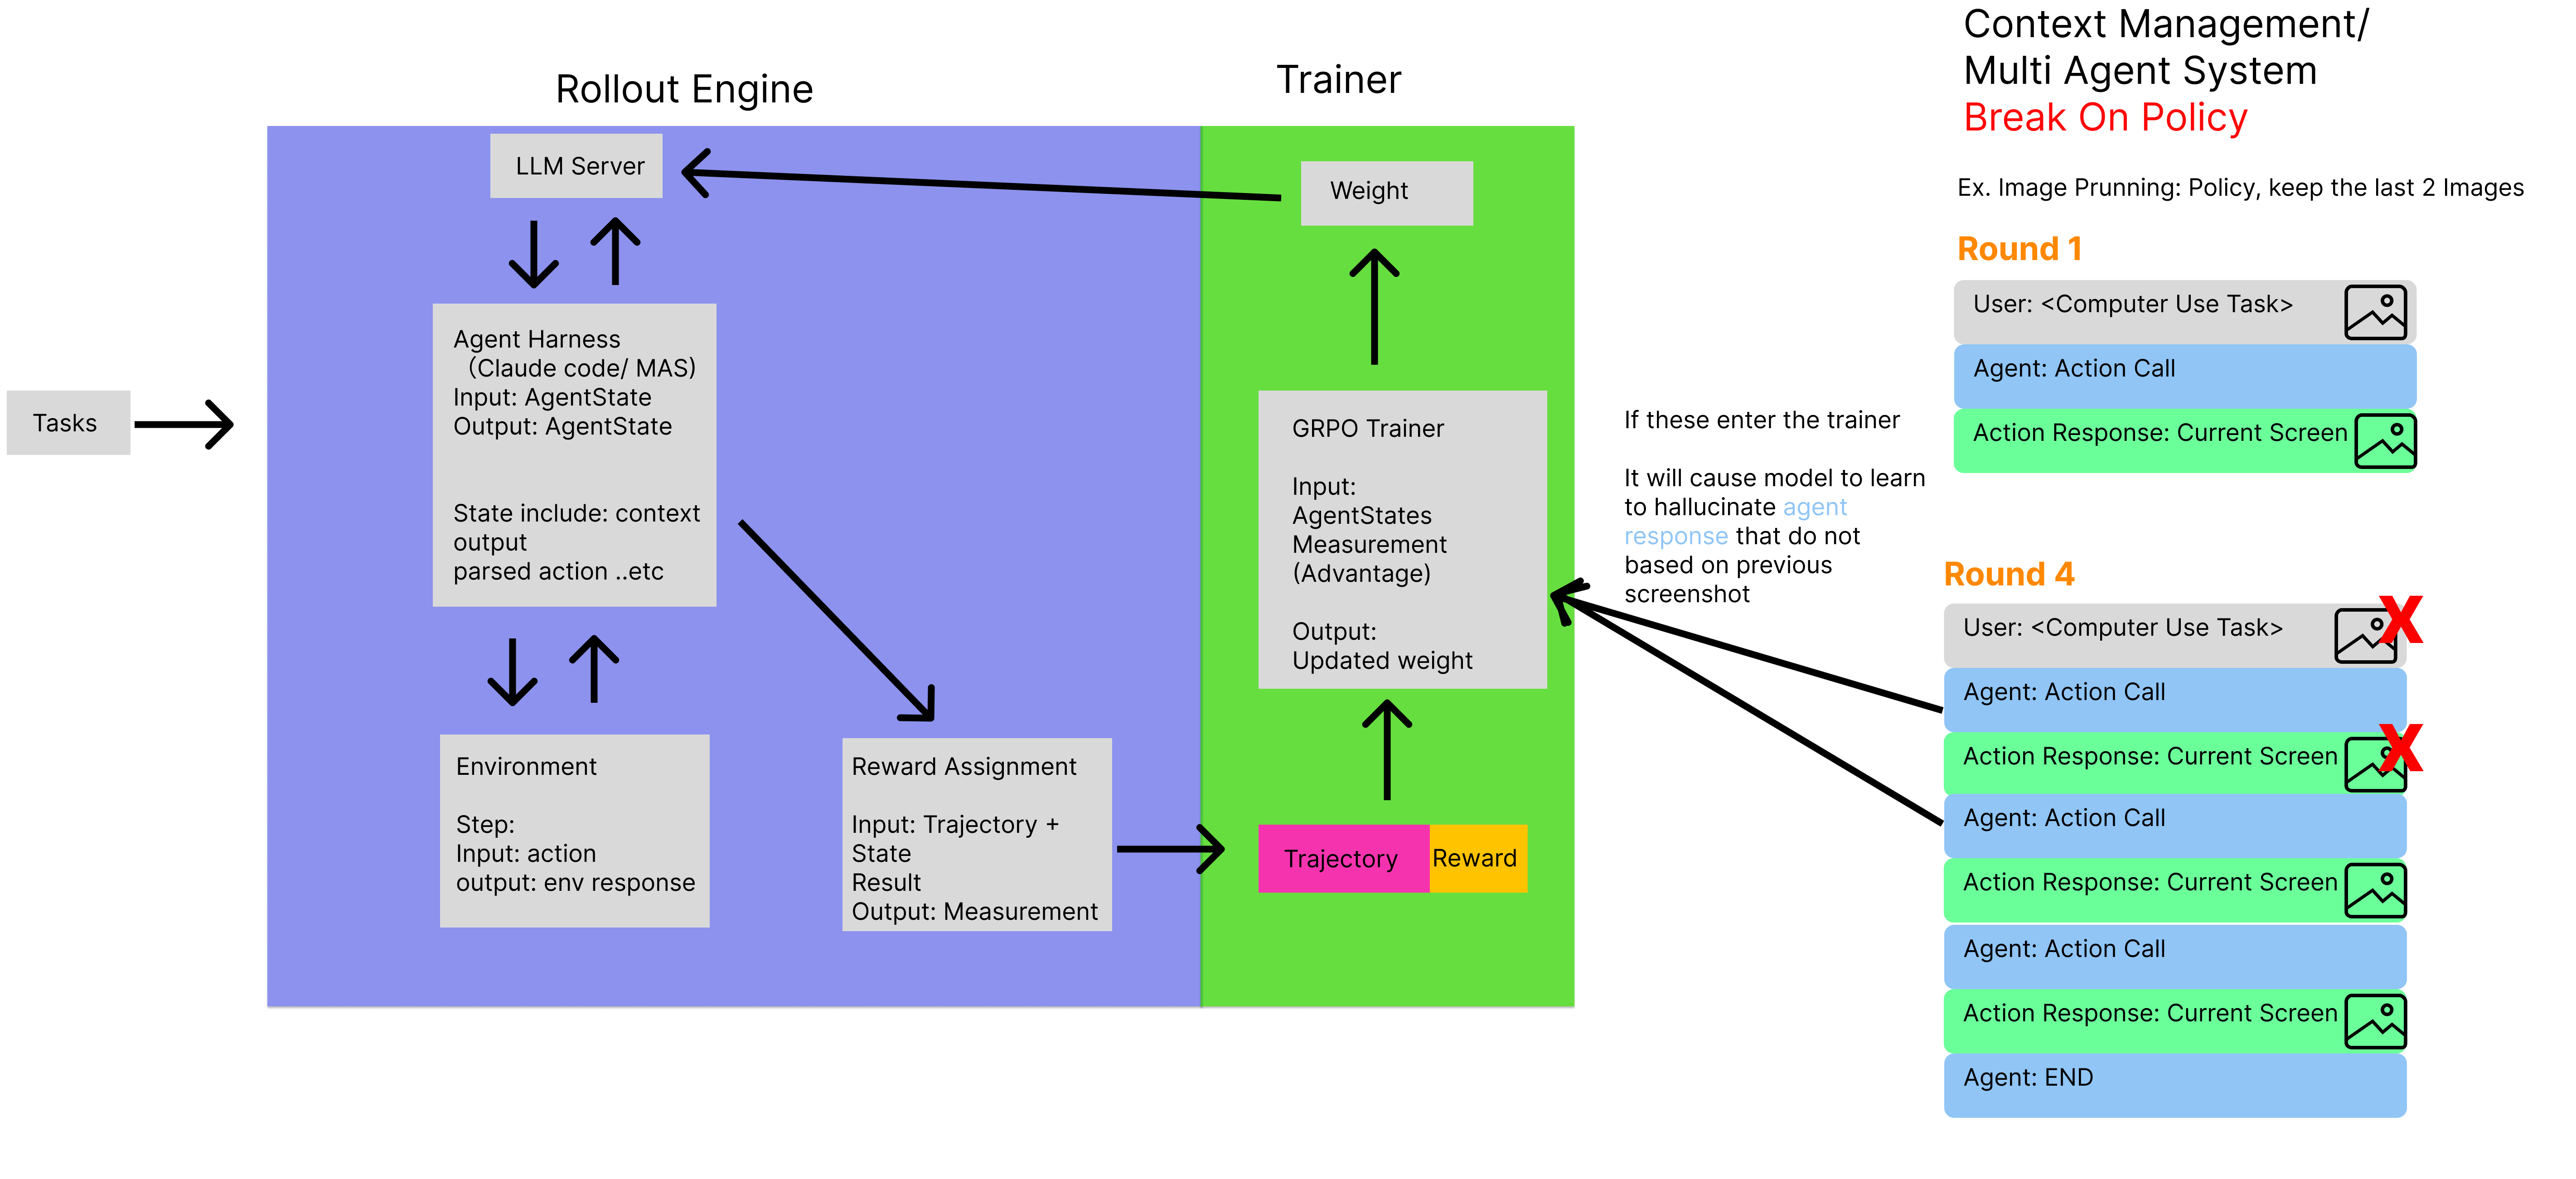
\includegraphics[width=0.96\textwidth]{figures/PreviousGRPO.png}

  \vspace{4mm}

  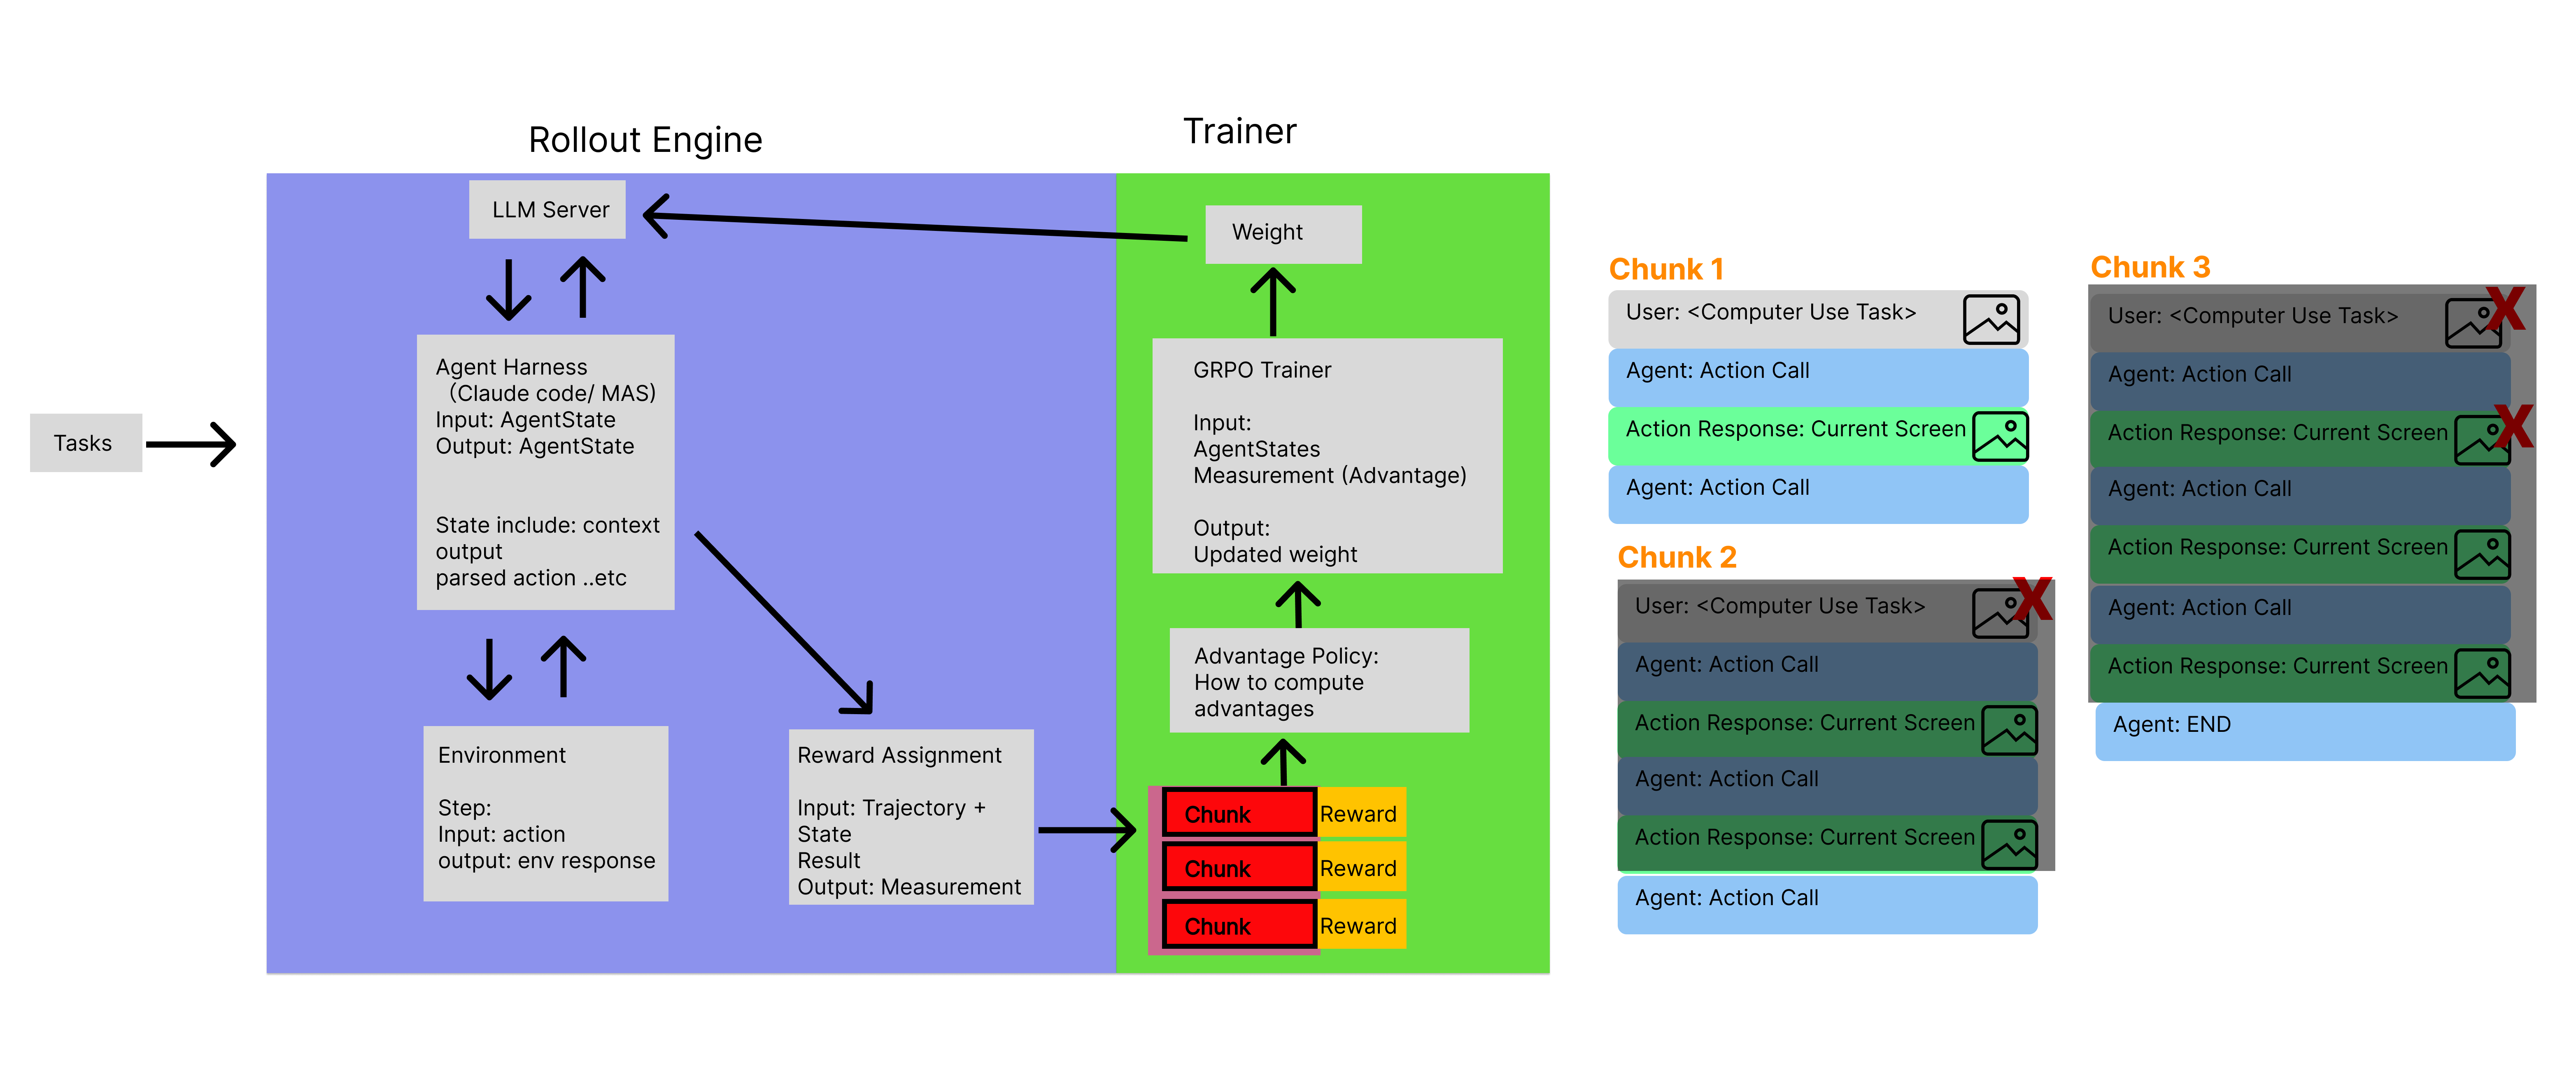
\includegraphics[width=0.96\textwidth]{figures/ChunkGRPO_PolarLike.png}
  \caption{Why single-trajectory reconstruction fails in a computer-use rollout that keeps
  only the last two screenshots. Top: treating the entire session as one GRPO sequence
  scores later actions under images that were absent when those actions were sampled.
  Bottom: a Polar-like construction starts a provenance-valid trace after each context
  change. The traces happen to share a terminal reward in this illustration, but separate
  trace rewards would be equally compatible with the on-policy construction. These are
  explanatory diagrams, not figures from the cited reports.}
  \label{fig:computer-use-grpo-trace-chunks}
\end{figure}

\clearpage
